\begin{figure}[H]
    \centering
    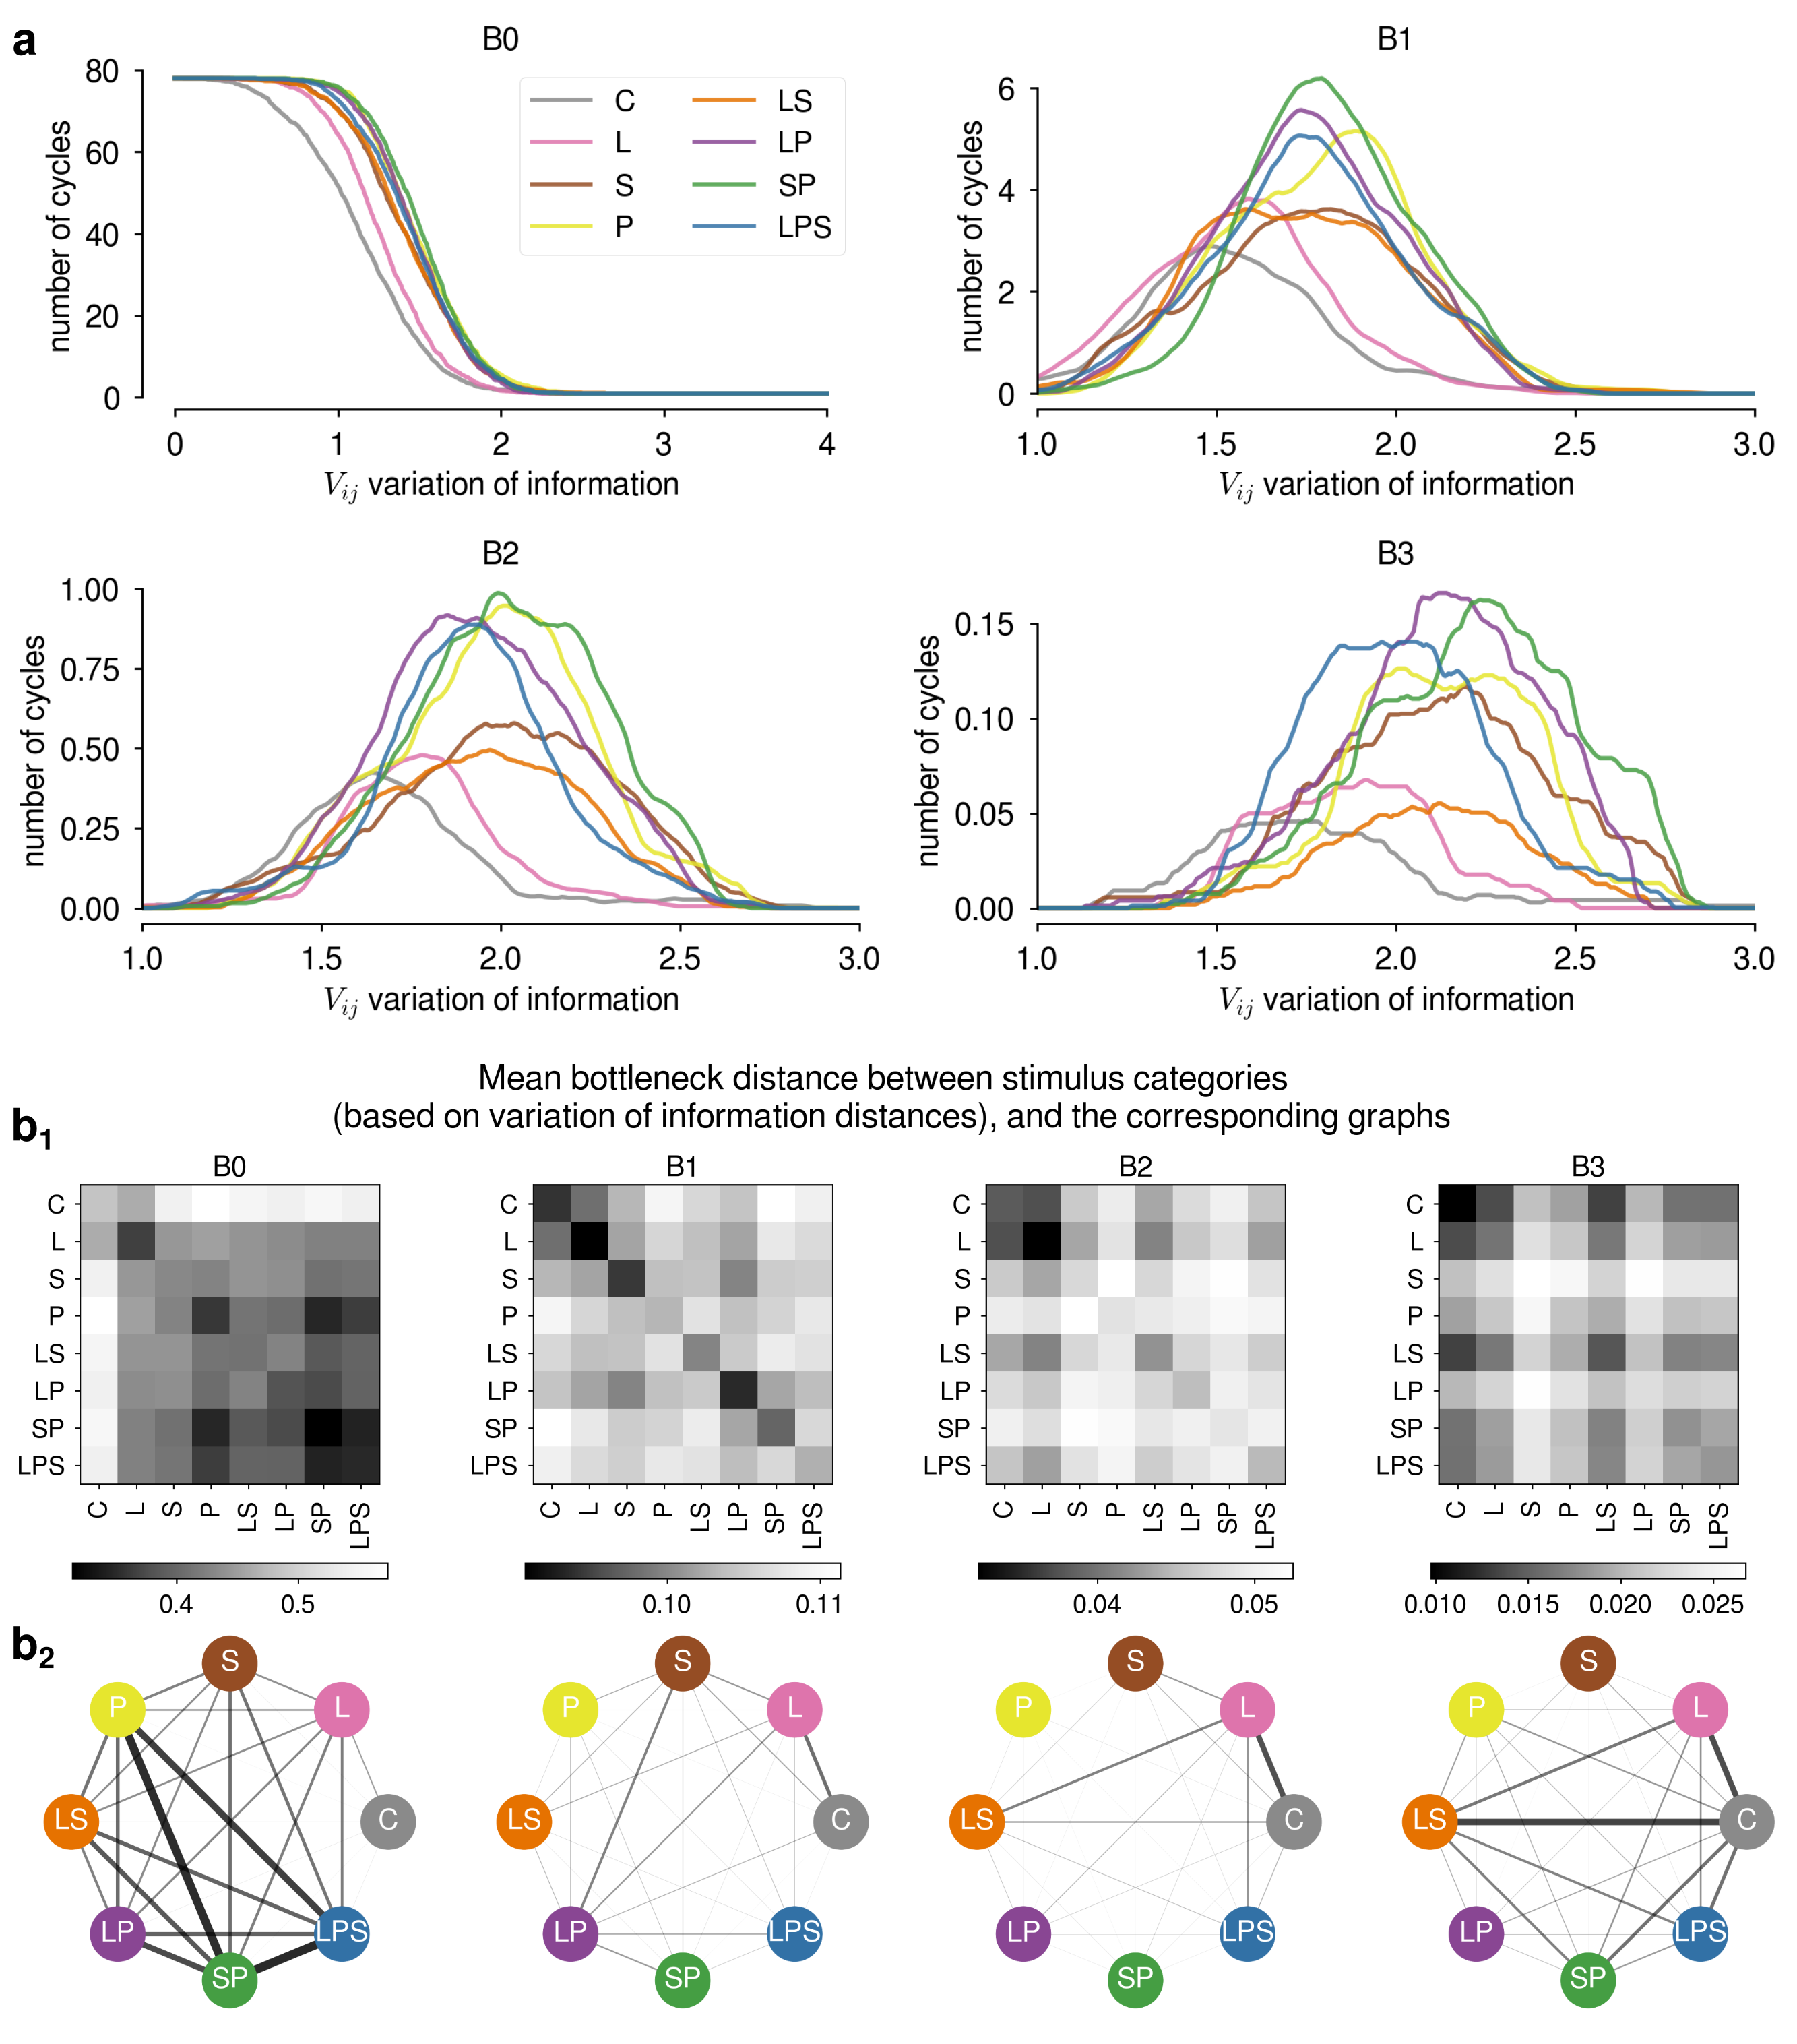
\includegraphics[width=0.7\textwidth,center]{../figures/report/Fig5.png}
    \caption{\label{fig:5}
    \textit{Comparison of Betti curves and bottleneck distances between Purkinje population topology of different stimulus conditions as a function of variation of information}.
    (\textbf{a}) Mean Betti curves as a function of $V_{ij}$  distance metric of the original data from variation of information matrix data. Colors are different stimulus categories. Different panels show different homology dimensions.
    (\textbf{b}) Mean bottleneck distance matrix (b$_1$) between different stimulus categories; and the graphs (b$_2$) constructed from converting these distance matrix to similarity matrix (i.e. thickness of edge means smaller bottleneck distance).
    }
\end{figure}

